\section{LTI-Systeme \schaum{25}}
\begin{center}
	\begin{tikzpicture}[scale=1, transform shape]
\node[input] (in) {};
\node[bigblock, right of=in] (lti) {LTI System};
\node[output, right of=lti] (out) {};

\draw [pfeil] (in) -- 
	node[above=0.5mm, name=sigma] {$\delta(t)$}
	node[below=0.5mm, name=xt] {$x(t)$}
	(lti);
\draw [pfeil] (lti) --
	node[above=0.5mm, name=ht] {$h(t)$}
	node[below=0.5mm, name=yt] {$y(t)$}
	(out);

\node[freetext, above of=sigma] (eins) {1};
\node[freetext, below of=xt] (Xw) {$X(\omega)$};
\node[freetext, above of=ht] (Hw) {$H(\omega)$};
\node[freetext, below of=yt] (Yw) {$Y(\omega)$};

\draw[doppelpfeil] (sigma) -- (eins);
\draw[doppelpfeil] (xt) -- (Xw);
\draw[doppelpfeil] (ht) -- (Hw);
\draw[doppelpfeil] (yt) -- (Yw);

% Formeln
\draw node[right=0mm of yt] {$=x(t)*h(t)$};
\draw node[right=0mm of Yw] {$=X(w)H(w)$};
\end{tikzpicture}
\end{center}

%\subsection{Eigenschaften von LTI-Systemen}
$ y(t) = T [ x(t)] \qquad $ Operator T erzeugt aus dem Eingangssignal $ x(t) $ das Ausgangssignal $ y(t)$. \\
\textbf{Linearität und Zeitinvarianz gelten!}\\
\begin{tabular}{lll}
	Bedingung für Linearität: & $T(x_1(t)+x_2(t))$ & $= T(x_1(t)) + T(x_2(t))$ \\
	& $T(ax(t))$ & $= a\cdot T(x(t))$\\
	Bedingung für Zeitinvarianz: & $y(t) = H(x(t))$ & $y(t-t_0) = H(x(t-t_0))$ \\
\end{tabular}

	\paragraph{Kausalität} Ein System ist kausal, wenn jedes Ausgangsignal durch ein vorhergehendes Eingangsignal gebildet wird.
\\

\subsection{Schrittfunktion - unit step}
	\begin{minipage}{10cm}
		$u(t) = \sigma(t) =	\begin{cases}
		  		 0 & \text{für } t < 0 \\
		  		 \frac{1}{2} \text{(praxis)}  \text{ oder undef. (math.)} & \text{für } t = 0 \\
		  		 1 & \text{für } t > 0
		  	\end{cases}
		$
		$\sigma(t) \FT \frac{1}{j\omega} + \pi\delta(\omega) = \Sigma(\omega)$
	\end{minipage}
	\begin{minipage}{8cm}
		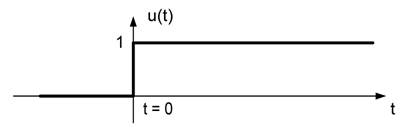
\includegraphics[width=6cm]{./bilder/unitstep.png}
	\end{minipage}

\subsection{Impulsfunktion - dirac delta function}
	\begin{minipage}{10cm}
		\begin{tabular}{l l}
		Definition & $\delta (t)=\begin{cases} 0 & t\ne 0\\\infty & t=0\end{cases}$ \qquad $\int\limits_{-\infty}^\infty \delta(t) \, \mathrm dt = 1 $\\
		\parbox{3cm}{Zusammenhang mit der $\sigma$-Funktion} & $\frac{d\sigma(t)}{dt}=\delta(t)$ \\
		\end{tabular}
		\[
			1 \FT 2\pi \delta(\omega) \qquad \delta(t) \FT 1(\omega)
		\]
	\end{minipage}
	\begin{minipage}{8cm}
		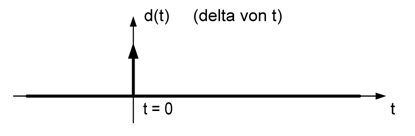
\includegraphics[width=6cm]{./bilder/diracimpulse.png}
	\end{minipage}

	\subsection{Impulsantwort \schaum{25-2.2B}}
		Die Impulsantwort $h(t)$ ist definiert als: $h(t) = T[\delta(t)] $ \\
		\hspace*{0.5cm} Bei kausalen Systemen: $h(t) = 0$ für $t < 0$ \\   
		\hspace*{0.5cm} Bei akausalen Systemen: $h(t) \neq 0$ für $t < 0$\\ 
		Die Antwort auf das Eingangssignal $x(t)$ berechnet sich: $y(t) = x(t) * h(t)$ \\
		
		Für weitere Details siehe Signale \& Systeme, bzw. IntTra Zusammenfassung.
		
		\subsubsection{Filtereigenschaft von $H(\omega)$}
			$ Y(\omega) = X(\omega) \cdot H(\omega)
				\qquad |Y(\omega)| = |X(\omega)| \cdot |H(\omega)|
				\qquad \varphi_{_Y}(\omega) = \varphi_{_X}(\omega) + \varphi_{_H}(\omega)$
		
		\subsubsection{Logarithmische Darstellung des Amplitudengangs}
			$ \qquad |H(\omega)| [dB] = 20 \cdot \log_{10}(|H(\omega)|)\qquad$
			\parbox{10cm}{So vereinfacht sich Berechnung der 
				Ausgangsamplitude:\\
				\hspace*{0.5cm}$ |Y(\omega)| [dB] = |X(\omega)|[dB] + |H(\omega)| [dB]$
			}

\subsection{Verzerrungen \schaum{26}}
	Signale werden in \"Ubertragungssystemen in vielfacher Wiese verformt (z.B. gefiltert, moduliert, gedämpft, entzerrt).
	\begin{multicols}{2}
		\textbf{Lineare Verzerrungen}
			\begin{itemize}
				\item Verursacht durch lineare (LTI) Systeme
				\item Das Superpositionsprinzip bleibt gültig
			\end{itemize}
			\columnbreak
			
		\textbf{Nicht-Lineare Verzerrungen}
			\begin{itemize}
				\item Verursacht durch nicht-lineare Systeme
				\item Oft schwierig modellierbar
				\item Oft nur numerisch berechenbar
			\end{itemize}
	\end{multicols}
	
	\subsubsection{Verzerrungsfreies LTI-System}
		\begin{minipage}[c]{6cm}
			Ein LTI-System ist verzerrungsfrei, wenn es das Eingangssignal zum Ausgang hin nur um $t_d$ verz\"ogert und/oder um einen Faktor K skaliert. 
		\end{minipage}
		$\quad \Longrightarrow \quad$
		\begin{minipage}[c]{4cm}
			$y(t) = K \cdot x(t-t_d)$  
			\\[0.2cm]
		%	\reflectbox{\rotatebox[origin=c]{270}{$\laplace$}}\\
			$Y(\omega) = K \cdot e^{-j\omega t_d} \cdot X(\omega)$\\[0.2cm]
			$\boxed{H(\omega) = K \cdot e^{-j\omega t_d}}$
		\end{minipage}
		$\Longrightarrow \quad$
		\begin{minipage}[c]{5cm}
			$|H(\omega)| = K$\\ \\
			$\varphi_{_H}(\omega) = -t_d \cdot \omega$
		\end{minipage}
	
	\subsubsection{Verzerrungen im LTI-System}
		\begin{minipage}[t]{7cm}
			\textbf{Amplitudenverzerrung}\\
				$\Rightarrow |H(\omega)|$ ist nicht konstant 
				
		\end{minipage}
		\begin{minipage}[t]{10cm}
			\textbf{Phasenverzerrung}\\
				$\Rightarrow \varphi_H (\omega)$ ist nicht linear von der Frequenz $\omega$ abhängig
		\end{minipage}


	\subsection{Filter \schaum{27}}
		\begin{multicols}{2}
			\begin{center}
				\begin{tabular}{|c|c|c|}
					\hline
					Tiefpass & Lowpass Filter & LPF \\
					\hline
					Hochpass & Highpass Filter & HPF \\
					\hline
					Bandpass & Bandpass Filter & BPF \\
					\hline
					Bandsperre & Bandstop Filter & BSF \\
					\hline
				\end{tabular}
			\end{center}
		\columnbreak
		\textbf{Ideale Filter} sind nicht realisierbar, da sie akausal sind.\\ \\
		\textbf{Kausale Filter} sind Ann\"ahrung an ideale Filter. \\ \\
		\textbf{TODO: Bilder von Filterdurchlasskurve einfügen}
	\end{multicols}

	\subsubsection{Bandbreite \schaum{28}}
	\begin{minipage}{7cm}
		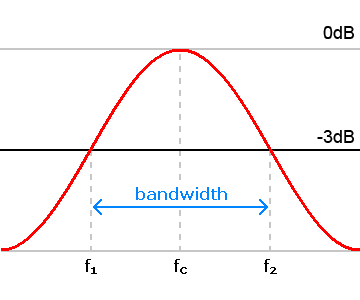
\includegraphics[width=6cm]{bilder/filter_bandbreite.png}
	\end{minipage}
	\begin{minipage}{11cm}
		Die Bandbreite ist nur für Tief- und Bandpassfilter definiert und bezieht sich auf das \textbf{einseitige} (reelle) Spektrum.
		\paragraph{LPF}	
			Die Bandbreite $W_B = 2 \pi B$ eines LPF entspricht der Frequenz, bei der $|H(\omega)|$ gegenüber $|H(0)|$ um $3 dB$ gedämpft ist
		\paragraph{BPF}	
			Filterbandbreite $W_B = 2 \pi B$ bei BPF entspricht der Differenz der (Kreis-) Frequenzen, bei denen Amplitudengang $|H(\omega)|$ gegenüber $|H(\omega_c)|$ um $3 dB$ gedämpft ist
	\end{minipage}


	\subsubsection{Quadraturfilter,Hilberttransformation \schaum{29}}
		\label{lti_quadratur}\label{lti_hilbert}
		Der Quadraturfilter ist ein Allpassfilter($ |H(\omega)| = 1 \quad \forall \; \omega $) mit
		Phasendrehung um $-\frac{\pi}{2};(-90^\circ)$ %\textbf{(differation)}
		.\\
		Ein Quadraturfilter ist technisch nur für einen beschränkten Bandbreitenbereich realisierbar.
		\[
			H(\omega) = \begin{cases}
             	e^{-j \frac{\pi}{2}} & \omega > 0 \\
             	e^{j \frac{\pi}{2}} & \omega < 0
             \end{cases} =
				-j \sgn(\omega)
				\qquad \Laplace \qquad h(t) = \frac{1}{\pi \cdot t}
		\]
		 \\
		 \textbf{Hilberttransformation} (Signal nach Quadraturfilter)
		\[
			\hat{X}(\omega) = H(\omega)X(\omega) = [-j \sgn(\omega)] X(\omega) \qquad \Laplace \qquad \hat{x}(t) = x(t) \ast \frac{1}{\pi \cdot t} = \frac{1}{\pi} \int\limits_{-\infty}^{+\infty} \frac{x(\tau)}{t-\tau} \diff \tau
		\]